\documentclass[pdftex,11pt,a4]{article}
\usepackage[parfill]{parskip}
\usepackage{lmodern}
\usepackage{amsmath, amsthm, amssymb}
\usepackage[usenames,dvipsnames]{xcolor}
\usepackage{tikz}
\usepackage{subcaption}
\usepackage{placeins}
\usepackage[pdftex]{graphicx}
\usepackage[T1]{fontenc}
\usepackage{calc}

\usepackage{listings}
\usepackage{inconsolata}
\lstset{basicstyle=\footnotesize\ttfamily,breaklines=true}
\lstset{language=Python, basewidth=0.5em,
  keywordstyle=\color{blue}, commentstyle=\color{Green}}

\def\code{\lstinline[basicstyle=\textsize\ttfamily]}

\newcommand{\sat}{\textsc{sat}}
\newcommand{\unsat}{\textsc{unsat}}

\begin{document}

\title{\textbf{Exploring Strategies for Performing Extended Resolution as a Preprocessing Step for SAT-Solving}}
\author{Eliot Ball}

\maketitle

\section*{Summary}

The summary.

\tableofcontents

\section{Introduction}

In a world increasingly driven by machines and other automated systems, bugs and mistakes made by the creators of these machines are expensive, and sometimes dangerous. In 1994, Intel was pressured into replacing a huge batch of its Pentium processors when it was discovered that the floating point unit within them was faulty, often returning inaccurate results. This recall cost Intel \$475 million. This type of mistake is often a huge problem for the parties involved, and it is easy to imagine truly disastrous outcomes if a mistake is made in the software for a missile guidance system, or the control systems for a car.

This raises the question of how to be sure that a system is correct -- answering the question, ``have we implemented what we intended to implement?'' Testing a system, by trying out all of the different types of situations we think it can reach, can only go so far. What if we fail to forsee some of the situations? Ideally, we would be able to prove beyond doubt that the system doesn't fail.

Bounded Model Checking is an approach to this where a system is encoded as a propositional formula that can be thought of as expressing the claim ``There is a counterexample, proving this system flawed, of length at most $k$'', for some given $k$. This formula is then checked to see whether it is satisfiable (``\sat'') using a \sat{}-solver. If the formula is \sat, then there is a counterexample of the desired length, which may be obtained by inspecting the values of the variables in satisfying assignment. If the formula is not satisfiable (it is \emph{unsatisfiable} or ``\unsat''), then we can be sure that there is not a counterexample of the desired length. The smallest possible $k$ guaranteeing that the system is completely correct (that there is no counterexample of any length) is called the \emph{completeness threshold}. In general, finding the completeness threshold is as hard as actually verifying the system, but many errors are shallow, and may be found with a low value of $k$. Therefore, using even a fairly small value can increase one's confidence in a system, even if one can still not be \emph{completely sure} that the system is correct.

Modern \sat{}-solvers operate on a machine-readable representation of formulas in \emph{conjunctive normal form} (CNF). A CNF formula is a conjunction of clauses, where each clause is a disjunction of literals:
\[(l_1 \vee l_2 \vee \cdots \vee l_j) \wedge (l_{j+1} \vee l_{j+2} \vee \cdots \vee l_k) \wedge \cdots \wedge (l_{m+1} \vee l_{m+2} \vee \cdots \vee l_n)\]
Each literal is either a variable or its negation. Note that this formula just requires one literal from each clause to be true.

For every propositional formula, there is an equivalent CNF formula, which can be found by repeated application of DeMorgan's laws, and the laws about distributivity and double negatives. Therefore \sat{}-solvers can effectively operate on all propositional formulas.

The most efficient modern \sat{}-solvers operate according to versions of the Davis-Putnam-Logemann-Loveland (DPLL) algorithm. The basis of this algorithm is essentially a depth-first search with backtracking of the whole space of partial assignments, looking for a full assignment that satisfies the formula. In the worst case, this type of exhaustive search would take $O(2^n)$ time to complete for a formula of $n$ variables. \sat{}-solvers can achieve much better performance in practice through the use of a number of heuristics. The DPLL algorithm introduced \emph{unit propagation}, which is the immediate assignment of the required value to any variables found on their own in a clause, and \emph{pure literal elimination}, which is the immediate assignment to any variable which is only found in one polarity in the whole formula (thereby making every clause containing that variable true) \cite{Davis:1962}. The latest \sat{}-solvers make heavy use of further optimisations such as faster data structures for the backtracking algorithm, better strategies for picking which variable to set at each step, and more advanced strategies for backtracking when a conflict is found \cite{Een:2003}. In particular, \emph{conflict driven clause learning} (CDCL) aims to infer a clause from a conflict which encapsulates in some sense the `reason' for the conflict, and causes the backtracking algorithm to fail more quickly on paths that would lead to failure for the same reason.

\section{Encodings and pre-processing}

For a given proposition about a system, there are many possible ways to encode that proposition in the CNF format accepted by the \sat{}-solver. For example, the ordering of the literals within each of the clauses, and the ordering of the clauses themselves may be changed. Because the \sat{}-solver has to make deterministic choices that are not prescribed in the DPLL algorithm, it may behave differently for different orderings. Therefore, even though $(l_0 \vee l_1) \wedge l_2 = (l_1 \vee l_0) \wedge l_2 = l_2 \wedge (l_0 \vee l_1)$, the \sat{}-solver may arrive at the solution to each of these formulas via a different sequence of steps.

Further, they may be multple ways to structure the representation of the system as a propositional formula. Suppose we are writing a CNF formula that is the result of applying an associative binary relation R to three objects $a$, $b$ and $c$. We could choose either $(a\mbox{ R }b)\mbox{ R }c$ or $a\mbox{ R }(b\mbox{ R }c)$. The \sat{}-solver may perform differently on each of these encodings. In real-world software verification, where we perform complex operations like multiplying and adding large binary numbers, there are many, many possible encodings, some of which perform drastically better than others. For example, a binary multiplier encoded as a table recording the result for every possible pair of operands performs much worse than one which borrows ideas from optimised hardware multipliers. [Is this true?]

The problem of picking an encoding for a proposition suggests the idea of pre-processing a formula before the \sat{}-solver is run. It may be possible to detect opportunities to re-structure a formula in such a way that the \sat{}-solver returns the result in less time. If the time saved by the \sat{}-solver is greater than the time taken to detect and apply the optimisations, then a net gain is made.

\section{Extended resolution}

The \emph{pigeonhole principle} states that, if $n > m$, it is impossible to place $n$ items in $m$ bins without any bins containing more than one item. We can attempt to verify this by encoding the contrapositive, ``it is possible to place $n>m$ items in $m$ bins without any bin containing more than one item'' as a propositional formula, and then showing that it is \unsat. As $n$ could be arbitrarily larger than $m$, we will actually show that the propositional formula encoding the assertion ``it is possible to place $n$ items in $n-1$ bins without any bin containing more than one item'' is \unsat. If it is impossible to place $n$ items in $n-1$ bins in this way, then it is certainly impossible to place even more items (since we have to place $n$ items in $n-1$ bins on the way), so this assertion suffices.

Let $P_{i,b}$ be a propositional variable standing for item $i$ being placed in bin $b$. Then we start by asserting that, for all items $1 \leq i \leq n$,
\[P_{i,1} \vee P_{i,2} \vee \cdots \vee P_{i,n-1}.\]
That is, for every item, it's either in bin 1, bin 2, \dots, or bin $n-1$ -- so every item is in a bin. Then we assert that, for every bin $1 \leq b \leq n-1$, for each pair of items $1 \leq i < j \leq n$,
\[\neg P_{i,b} \vee \neg P_{j,b}.\]
That is, for each bin, for each pair of items, one or other of those items is not in the bin -- so no pair of items is in the same bin. Together these clauses assert that it is possible to place $n$ items in $n-1$ bins without more than one item in any bin. This formula is \unsat.

One way of proving that this formula is \unsat{} is to provide a resolution refutation. Where clauses are respresented as sets of literals (e.g. $a \vee \neg b = \{a, \neg b\}$), the resolution rule works as follows.

\begin{table}[h]
  \begin{tabular}{lll}
    {\bf 1} & $C_1 \cup \{L\}$ & premise \\
    {\bf 2} & $C_2 \cup \{\neg L\}$ & premise \\
    {\bf 3} & $C_1 \cup C_2$ & res {\bf 1}, {\bf 2}
  \end{tabular}
\end{table}
\FloatBarrier

For example, we can use resolution to prove the pigeonhole principle for the easy $n = 2$ case:

\begin{table}[h]
  \begin{tabular}{lll}
    {\bf 1} & $\{P_{1,1}\}$ & premise \\
    {\bf 2} & $\{P_{2,1}\}$ & premise \\
    {\bf 3} & $\{\neg P_{1,1}, \neg P_{2,1}\}$ & premise \\
    {\bf 4} & $\{\neg P_{2,1}\}$ & res {\bf 1}, {\bf 3} \\
    {\bf 5} & $\bot$ & res {\bf 2}, {\bf 4}
  \end{tabular}
\end{table}
\FloatBarrier

This is, in fact, a \emph{tree resolution} proof, because no clause is antecedent to more than one other clause. Unfortunately, for sufficiently large $n$, a tree resolution proof of the pigeonhole principle for $n$ items requires $2^{\Omega(n)}$ steps, suggesting that tree resolution may not be the best proof system with which to prove the pigeonhole principle.
% Haken 1985
However, runs of DPLL-based \sat{}-solvers on \unsat{} formulas correspond to tree resolution refutations of the formula, which suggests that such \sat{}-solvers will exhibit low performance on instances of the pigeonhole principle, and perhaps other similar formulas.
% Handbook of constraint programming
This raises the question of whether there is a more powerful system that allows a sub-exponential length proof, and thus better performance by a DPLL-based \sat{}-solver on this type of instance. One such system is \emph{extended resolution}.

% Suggests using a more powerful system

Extended resolution adds an additional rule beyond the resolution rule. Given a pair of literals $l_1$ and $l_2$ from the propositional formula, and a fresh variable $x$, we may introduce a new set of clauses representing $x \leftrightarrow l_1 \vee l_2$ \cite{Tseitin:1983}.
% Tsetin - On the complexity of derivation in propositional calculus
The set of clauses representing this addition is

\begin{equation*}
  \begin{align*}
    x \leftrightarrow l_1 \vee l_2 &= (x \to (l_1 \vee l_2)) \wedge (l_1 \to x) \wedge (l_2 \to x) \\
          &= (\neg x \vee l_1 \vee l_2) \wedge (\neg l_1 \vee x) \wedge (\neg l_2 \vee x).
  \end{align*}
\end{equation*}

Extended resolution suggests itself as a good candidate for a more powerful system because it permits a polynomial-length proof of the pigeonhole principle \cite{Cook:1976}.

A conventional proof of the pigeonhole principle works by induction on $n$. First, it can easily be shown that it's not possible to assign 2 items to 1 bin without the sole bin containing more than one item (it will have to contain both!), as we did by resolution above. We will phrase this as the lack of an injective mapping from $\{1,2\}$ to $\{1\}$. Then, for the inductive step, we show that if there is a mapping from $\{1,2,\ldots,n\}$ to $\{1,2,\ldots,n-1\}$, then there is a mapping from $\{1,2,\ldots,n-1\}$ to $\{1,2,\ldots,n-2\}$. We do this by supposing that $\phi$ is an injective mapping from $\{1,2,\ldots,n\}$ to $\{1,2,\ldots,n-1\}$, in which case
\[\phi'(i) = \begin{cases}
\phi(n) & \mbox{if } \phi(i) = n-1, \\
\phi(i) & \mbox{otherwise}
\end{cases}\]
is an injective mapping from $\{1,2,\ldots,n-1\}$ to $\{1,2,\ldots,n-2\}$. Intuitively, $\phi'$ maps everything in the same way as $\phi$, except that the mappings \emph{from} $n$ and \emph{to} $n-1$ are merged, allowing those numbers to be deleted (see Figure \ref{fig:php-induction}). Since there isn't a mapping for $n=2$, by contradiction there can't be one for $n=3$, and therefore there is none for $n=4$, and so on.

\begin{figure}[h]
  \begin{subfigure}[H]{0.5\textwidth}
    \centering
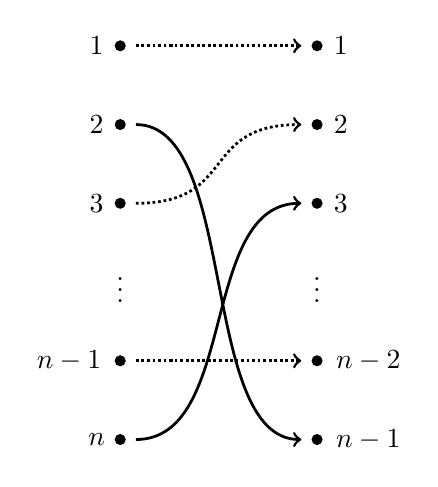
\begin{tikzpicture}
\fill (1,5) circle (2pt);
\fill (1,4) circle (2pt);
\fill (1,3) circle (2pt);
\fill (1,1) circle (2pt);
\fill (1,0) circle (2pt);

\fill (3.5,5) circle (2pt);
\fill (3.5,4) circle (2pt);
\fill (3.5,3) circle (2pt);
\fill (3.5,1) circle (2pt);
\fill (3.5,0) circle (2pt);

\node[draw=none] at (1,2) {$\vdots$};
\node[draw=none] at (3.5,2) {$\vdots$};

\node[draw=none] at (0.7,5) {1};
\node[draw=none] at (0.7,4) {2};
\node[draw=none] at (0.7,3) {3};
\node[draw=none] at (0.35,1) {$n-1$};
\node[draw=none] at (0.7,0) {$n$};

\node[draw=none] at (3.8,5) {1};
\node[draw=none] at (3.8,4) {2};
\node[draw=none] at (3.8,3) {3};
\node[draw=none] at (4.15,1) {$n-2$};
\node[draw=none] at (4.15,0) {$n-1$};

\draw[line width=1pt, densely dotted] [->] (1.2,5) .. controls (2.5,5) and (2,5) .. (3.3,5);
\draw[line width=1pt] [->] (1.2,4) .. controls (2.5,4) and (2,0) .. (3.3,0);
\draw[line width=1pt, densely dotted] [->] (1.2,3) .. controls (2.5,3) and (2,4) .. (3.3,4);
\draw[line width=1pt, densely dotted] [->] (1.2,1) .. controls (2.5,1) and (2,1) .. (3.3,1);
\draw[line width=1pt] [->] (1.2,0) .. controls (2.5,0) and (2,3) .. (3.3,3);
\end{tikzpicture}

    \caption{An example mapping $\phi$}
  \end{subfigure}
  %
  \begin{subfigure}[H]{0.5\textwidth}
    \input{right-pigeonhole.tex}
    \caption{The derived $\phi'$}
  \end{subfigure}
  \caption{An illustration of the inductive step in proving the pigeonhole principle}
  \label{fig:php-induction}
\end{figure}

Suppose we have the clauses restricting the values of $P_{i,b}$ for some instance of the pigeonhole principle, as given above. These clauses, if they are satisfiable, imply some mapping $\phi$. We now introduce new propositional variables $Q_{i,b}$, with $1 \leq i \leq n-1$ and $1 \leq b \leq n-2$, which, if satisfiable, describe the corresponding mapping $\phi'$. We set

\begin{equation*}
  \begin{align*}
    Q_{i,b} &= P_{i,b} \vee (P_{i,n-1} \wedge P_{n,b}) \\
      &= (P_{i,b} \vee P_{i,n-1}) \wedge (P_{i,b} \vee P_{n,b}),
  \end{align*}
\end{equation*}

which just says that the new mapping of a particular item ($Q_{i,b}$) either matches the old one ($P_{i,b}$) or it represents that merge between the mappings from $n$ and to $n-1$ ($P_{i,n-1} \wedge P_{n,b}$). This can be achieved by performing two extensions per variable $Q_{i,b}$:

\begin{equation*}
  \begin{align*}
    Q_{i,b} &\leftrightarrow P_{i,b} \vee P_{i,n-1} \\
    Q_{i,b} &\leftrightarrow P_{i,b} \vee P_{n,b}
  \end{align*}
\end{equation*}

From this new (polynomial-size) set of clauses, and the clauses given by the instance of the pigeonhole principle for $n$ items, we can obtain, by a polynomial number of resolutions, the following clauses:

\begin{table}[h]
  \begin{tabular}{rll}
        & $Q_{i,1} \vee Q_{i,2} \vee \cdots \vee Q_{i,n-2}$ & for $1 \leq i \leq n-1$, \\
    and & $\neg Q_{i,b} \vee \neg Q_{j,b}$ & for $1 \leq b \leq n-2$ and $1 \leq i < j \leq n-1$.
  \end{tabular}
\end{table}
\FloatBarrier

These clauses describe the pigeonhole principle for $n-1$ items. Repeating this process of extension and resolution $O(n)$ times gives a polynomial-length proof of the pigeonhole principle.

\section{Strategies for extension}

We have seen by the example of the pigeonhole principle that adding extension to the resolution proof system can sometimes permit polynomial-length proofs of assertions that would otherwise require exponential length. Since tree resolution proofs correspond to runs of DPLL-based \sat{}-solvers, adding the ability to perform extension in the process of \sat{}-solving can potentially improve the performance of \sat{}-solvers.

In 2010, a restriction of extended resolution was demonstrated which may be used to create a \sat{}-solver which, in some cases, outperforms ones that do not use extension \cite{Audemard:2010}. The authors note that, prior to their paper, no \sat{}-solver based on extended resolution had been proposed, because ``it is hard to devise a heuristic that introduces variables that are likely to help find a short refutation''. In other words, it is unclear which extensions to perform, in order to increase performance. They propose restricting the situations where extension may be performed to those where there are two clauses, $C_1 = l_1 \vee \alpha$ and $C_2 = l_2 \vee \beta$, where neither $\alpha$ nor $\beta$ contain negations of any literals contained in the other, in which case extension may be performed to introduce $z \leftrightarrow \neg l_1 \vee \neg l_2$. The aim of doing so is to avoid redundancy in any later sequence of resolutions producing a new pair of clauses which essentially only differ in that one includes $l_1$ and the other $l_2$. They describe a performant way of implementing this strategy that outperformed state-of-the-art \sat{}-solvers on instances from recent competitions.

In 2015, a group of students explored the possibility of using \emph{common subexpression elimination} (CSE) in various ways to improve the performance of \sat{}-solving \cite{Yan:2015}. They suggest eliminating certain repeated subexpressions by introducing new variables using a generalised version of extension (although they do not actually mention extended resolution themselves). If $\{l_1, l_2, \ldots, l_n\}$ is a set of literals from a propositional formula and $x$ is a fresh variable, then we can introduce the clauses necessary to establish
\[x \leftrightarrow l_1 \vee l_2 \vee \cdots \vee l_n\]
and then, in any clause containing all of $l_1, l_2, \ldots, l_n$, delete those literals, and add $x$. Three methods are given for choosing which subexpressions to eliminate. In the first, the common subexpressions are chosen such that, after they are eliminated, the problem is of minimal size. The authors conjecture that this problem is NP-hard, and give two approximate algorithms. One is based on replacing subexpressions that are found with frequency above a given threshold, and the other is based on the LZW string-compression algorithm. All of these strategies are implemented as a pre-processing step before running the \sat{}-solver. This approach is attractive because of its simplicity, and the authors find an improvement in performance in some cases.

For this project, I hypothesise that, for some propositional formulas arising in real-world model checking, there are sets of substitutions of repeated subclauses with size 2 or 3 (that is, there are pairs or triplets of literals which appear in multiple clauses) which can be replaced by extension with a single variable, leading to an improvement in the performance of the \textsc{MiniSat} solver on those instances. I investigate this by attempting to use a genetic algorithm to find such sets of substitutions.

\section{Genetic algorithms}

A \emph{genetic algorithm} is a search algorithm that mimics natural selection. In the most basic form of the algorithm, sufficiently long binary strings are mapped onto the search space, and then an initial population of random strings is created. Each of the strings is scored according to the fitness of the corresponding item in the search space, and then a sample of the most highly-scored strings is taken. From this sample, a new population the same size as the original is created, by taking random pairs of strings from the sample and combining them in a specific way (see below). This process of scoring, sampling, and combining is repeated a nubmer of times, in the hope of finding a member of the search space with high fitness.

In the step where a new population is being generated from the high-fitness sample, the new population members are usually generated according to the following algorithm (See Figure \ref{fig:genetic-algo}):

\begin{enumerate}
  \item {\bf Selection:} Randomly choose two \emph{parents} $a$ and $b$ from the high-fitness sample.
  \item {\bf Crossover:} Where $n$ is the length of the strings, pick some integer $k$ such that $0 \leq k \leq n$, and then combine the two parent strings to create the new member $m = a[0 \ldots k) \parallel b[k \ldots n)$.
  \item {\bf Mutation:} Randomly flip some of the bits in $m$ and then add it to the new population.
\end{enumerate}

\begin{figure}[h]
  \centering
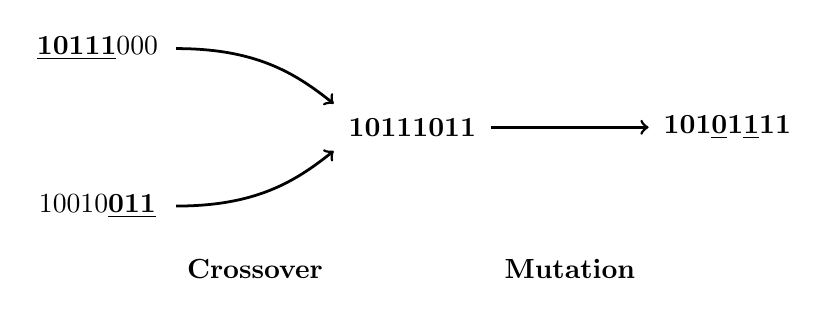
\begin{tikzpicture}
  \node[draw=none] at (0,1) {10010\underline{\bf 011}};
  \node[draw=none] at (0,3) {\underline{\bf 10111}000};

  \node[draw=none] at (4,2) {\bf 10111011};
  \node[draw=none] at (2,0.2) {\bf Crossover};

  \node[draw=none] at (8,2) {\bf 101\underline{0}1\underline{1}11};
  \node[draw=none] at (6,0.2) {\bf Mutation};

  \draw[line width=1pt] [->] (1.0,3) .. controls (2.0,3.0) and (2.5,2.7) .. (3.0,2.3);
  \draw[line width=1pt] [->] (1.0,1) .. controls (2.0,1.0) and (2.5,1.3) .. (3.0,1.7);
  \draw[line width=1pt] [->] (5.0,2) to (7.0,2);
\end{tikzpicture}

  \caption{An illustration of the generation of a new member from a pair of parents in a genetic algorithm}
  \label{fig:genetic-algo}
\end{figure}

The aim of the crossover part of the algorithm is to allow good features that are developed in separate members of the population to be combined as ``building blocks'', sometimes leading to a member of the population that is stronger than either of the original members \cite{Goldberg:1989}. In some variations on the basic genetic algorithm, multiple ``cuts'' are made so that more than two members of the population may be combined, but this hasn't been found to produce better final outcomes in most cases, and can lead to premature convergence, owing to a loss of genetic diversity in the population \cite{Esquivel:1997}.

The aim of the mutation part of the algorithm is to allow the exploration of ``nearby'' members of the population. If the search space is sufficiently smooth with respect to the fitness function, then this leads to a hillclimbing effect. This also means that care must be taken with the encoding of solutions as bit vectors, and when setting the rate of mutation, since certain encodings or rates of mutation may not lead to a sufficiently similar ``neighbouring'' solutions for the hillclimbing effect to work correctly \cite{Taher:2013}. In general, the probability of any bit in a member of the population being flipped should not be above 0.05, and with a mutation rate below that threshold, the population size should be between approximately 30 and 100 \cite{Grefenstette:1986}.

There are several different strategies for the selection phase, where the high-fitness sample is chosen \cite{Thierens:1994}. The simplest is \emph{truncation selection}, which is the outcome of sorting the population by fitness, and taking the best $k$ members, for some $k$. An alternative approach is \emph{fitness proportionate selection}, also called \emph{roulette-wheel selection}, where we calculate the fitness of each individual, and then assign each individual some part of the $[0,1]$ interval, so that the size of each individual's section of the interval is proportional to its fitness. Then a random point in the $[0,1]$ interval is picked, and the corresponding member of the population is added to the high-fitness sample. This is repeated $k$ times, where $k$ is the desired size of the high-fitness sample. Both of these strategies generally perform well, but fitness proportionate selection can run in to problems at later stages of execution when the fitness values of the population are similar, as it might not provide enough selection pressure to improve the population \cite{Whitley:1989}. As the fitness values of members of the population in this project are indeed likely to be similar, I chose to use truncation selection.

% Elitism

\section{Technical implementation}

In the technical implementation of this project, I obtained a number of benchmarks that come from real-world bounded model checking. The benchmarks come from implementations of the Newton-Raphson method, polynomial approximations of sine, and squaring of floating-point numbers. To execute the genetic algorithm on a given benchmark, we follow this algorithm:

\begin{samepage}
  \begin{enumerate}
    \item Find, and number, all of the repeated subclauses of size 2 or 3.
    \item Generate an initial population of 50 bit vectors, each having one bit per subclause.
    \item For each member of the population, create a new benchmark file by performing the required extensions.
    \item Run \textsc{MiniSat} on each member of the population, recording the time taken.
    \item If the average fitness for the whole population has converged, terminate.
    \item Rank members of the population by their \textsc{MiniSat} time, and take the best half.
    \item Generate a new population of 50 comprising the best half of the previous population, along with another half created from that half by crossover and mutation.
    \item Go to Step 3.
  \end{enumerate}
\end{samepage}

Finding all of the repeated subclauses of size 2 or 3 could be done in many ways. For example, simply passing over the file counting the number of occurrences of each subclause would work, particularly when each clause is small. This problem has been studied relatively extensively within the field of database mining, where fast algorithms such as the \emph{Apriori algorithm} have been discovered, which scale up effectively to very large datasets \cite{Agrawal:1994}. A detailed investigation of these algorithms is beyond the scope of this project, since the goal is simply to determine whether there are sets of subclause replacements which improve \sat{}-solver perfomance. For Step 1 of the above algorithm, I simply call an existing program that uses the Apriori algorithm \cite{Borgelt:2003}.

\begin{figure}[p]
  %\hspace*{-1cm}%
\begin{minipage}{\textwidth+2cm}
  \begin{lstlisting}
class Population():
  def __init__(self, string_length, size=50, select_best=25):
      self.size = size
      self.select_best = select_best
      self.members = [[random_bit() for j in xrange(string_length)]
                      for i in xrange(size - 2)]
      self.members += [[True for i in xrange(string_length)]]
      self.members += [[False for i in xrange(string_length)]]

  def get_best_few(self, scoring_function):
      scores = []
      for member in self.members:
          this_score, other_data = scoring_function(member)
          scores += [{
              "member": member,
              "score": this_score,
              "other_data": other_data
          }]
          scores.sort(key=lambda s: s["score"])  # smaller is better
      total_fitness = sum([score["score"] for score in scores])
      return (total_fitness, [i["member"] for i in scores[:self.select_best]], scores)

  def improve(self, scoring_function, mutation_probability):
      total_fitness, best_few, all_scores = self.get_best_few(scoring_function)
      self.generate_new_members(best_few, mutation_probability)
      return total_fitness

  def generate_new_members(self, best_few, mutation_probability=0.01):
      self.members = best_few
      for member_count in xrange(len(best_few), self.size):
          left_parent = random.choice(best_few)
          right_parent = random.choice(best_few)
          # Crossover
          assert len(left_parent) == len(right_parent)
          crossover_point = random.randint(0, len(left_parent))
          new_member = left_parent[:crossover_point] \
              + right_parent[crossover_point:]
          # Mutation
          for i in xrange(len(new_member)):
              if random.random() < mutation_probability:
                  new_member[i] = not new_member[i]
          self.members += [new_member]
  \end{lstlisting}
\end{minipage}%
%\hspace*{-1cm}%

  \caption{The essential methods of the Population class. (Code that performs logging, and other ancillory functions like converting the population to and from strings, is not included here as it is immaterial to the behaviour of the program.)}
  \label{fig:population-class}
\end{figure}

For the genetic algorithm, the population is handled by the \code{Population} class (see Figure \ref{fig:population-class}). The initial population is generated in the \code{__init__} method by creating 48 (or 2 less than \code{population_size} if that is not 50) random bit vectors of the appropriate length. The bit vectors are represented as lists of boolean values. This is not very efficient in memory, but it doesn't matter because the population is quite small.




% Performing extension
% Measuring performance
% Extension inside a GA
% Execution of algorithm



\section{Analysis of results}

\begin{itemize}
  \item Analysis
\end{itemize}

\section{Conclusion}

\FloatBarrier
\bibliography{report}
\bibliographystyle{apalike}

\end{document}
